\subsection{Приведение грамматики к НФХ.}

\deff{Грамматика в нормальной форме Хомского}, если любое правило имеет вид:
$$A \xrightarrow{} BC \quad A \xrightarrow{} c$$
А также, возможно правило из $S\xrightarrow{} \varepsilon$, но тогда $S$ не встречается в правых частях правил.

Давайте научимся приводить грамматику в нормальный вид Хомского:
\begin{enumerate}
    \item Для всех терминалов заведем их личные нетерминалы и добавим правило $N_c \xrightarrow{ }c$, а также заменим во всех правилах $c$ на $N_c$. У нас остались такие правила с нетерминалами: 
    \begin{enumerate}
        \item $A \xrightarrow{} \varepsilon$, 0 нетерминалов. $\varepsilon$-правила
        \item $A \xrightarrow{} B$, 1 нетерминал. Цепные правила.
        \item $A \xrightarrow{} BC$, 2 нетерминала.
        \item $A \xrightarrow{} N_1\ldots N_k, k \geq 3$. Длинные правила.
    \end{enumerate}
    Осталось победить 3 вида правил.
    \item Победим правила. Начнем с длинных. Возьмем правило$A \xrightarrow{} N_1\ldots N_k, k \geq 3$. 
    
    Заменим его на правила:
    $A \xrightarrow{} N_1 Y_1, Y_1 \xrightarrow{} N_2 Y_2, Y_{k-2}\xrightarrow{} N_{k-1}N_k$. Победили!

    \item Удалим $\varepsilon$ правила. Найдем все эпсилон порождающие терминалы (из которых можно вывести $\varepsilon$). Как такие искать?

    Перебираем все правила, если из правила мы получаем в правой стороне все эпсилон порождающие нетерминалы, то отметим текущее правило эпсилон порождающим. Будем продолжать так, пока изменения не прекратятся. 

    Выкинем все эпсилоны. $S'$ - новый стартовый символ. Если $S$ - эпсилон порождающий, то $S'\xrightarrow{} S, S'\xrightarrow{} \varepsilon$. И выкинем эпсилон правила.

    Победили второго врага!
    \item Остались цепные правила. Сделаем транзитивное замыкание по ним. Оставим только нецепные правила. Все работает.
\end{enumerate}
В чем прикол НФХ? Дерево разбора бинарное!!!    

\subsection{Алгоритм Коко-Янгера-Касами (КЯК или CYK)}

\sout{Алгоритм тупой динамики}

Алгоритм Кока-Янгера-Касами --- алгоритм, позволяющий по слову узнать, выводимо ли оно в заданной КС-грамматике в нормальной форме Хомского. Любую КС-грамматику можно привести к НФХ, как мы показали ранее, поэтому алгоритм является универсальным для любой КС-грамматики.

Пусть у меня есть слово $x$ длины $n$. Cделаем динамику:

$d_A[l][r]$ - можно ли из $A$ вывести подстроку $x[l\ldots r-1]$

Тогда для $r-l >1$, будет выполнено:
$$d_A [l][r] = \bigvee\limits_{A\xrightarrow{} BC} \bigvee\limits_{k=l+1}^{r-l}(d_B[l][k] \wedge d_C[k][r])$$ где $\bigvee$ это логическая дизъюнкция.

Теперь порядок вычисления. Вычисляем по возрастанию длины. Ответ лежит в $d_S[0][n]$. Первый слой задаем руками.

\subsection{МП автомат}

Автомат с магазинной памятью -  это конечный автомат, который использует стек для хранения состояний.

Есть автомат и стек. $z_0$ - маркер дна. 



МП автомат = стековая машина = Push-down Automaton. У него есть стек.

Есть 2 вида стеков:
\begin{enumerate}
    \item по пустому стеку.
    \item по допускающему состоянию.
\end{enumerate}

Пример не детерминированного МП-автомата для языка $0^n1^n$:

\begin{center}
   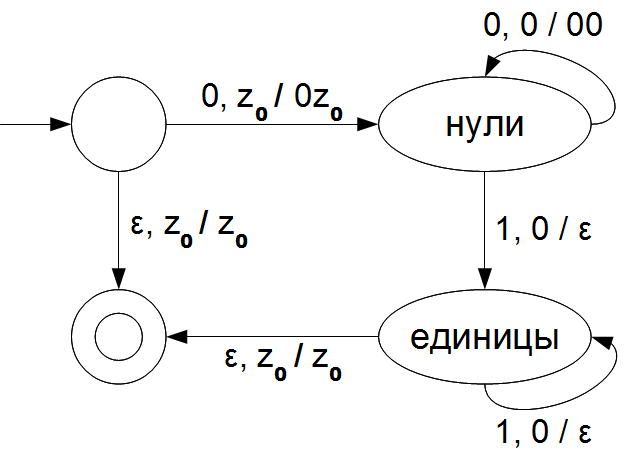
\includegraphics[width=12cm]{assets/12_3_1.png}
\end{center}